% $Id: ESMF_infradataoverview.tex,v 1.12 2004/04/15 20:19:18 cdeluca Exp $

\section{Overview of Infrastructure Data Structures}

The ESMF infrastructure data classes are part of the framework's 
hierarchy of structures for handling Earth system model data and 
metadata on parallel platforms.  The hierarchy is in complexity; the simplest 
data class in the infrastructure represents a distributed array and the most
complex data class represents a set of physical fields that are discretized 
on the same grid.  Data class methods are called both from user 
written code and from other classes internal to the framework.  

ESMF data classes are useful because they provide a 
standard, convenient way for developers to collect information 
related to model or observational data.  The information assembled 
includes a data pointer, a set of associated attributes (e.g. units, 
although attributes can also be user-defined), and a 
description of an associated grid.  The same set of information within 
an ESMF data object can be used by the framework to arrange 
intercomponent data transfers, to perform I/O, for communications
such as gathers and scatters, for simplification of interfaces 
within user code, for debugging, and for other functions.  
This unifies and organizes codes overall so that the user need not,
for example, define different representations of metadata for the
same field for I/O and for component coupling.  

Since it is critical that users be able to introduce ESMF into their
codes easily and incrementally, ESMF data classes can be created based 
on native Fortran pointers.  Likewise, there are methods for retrieving 
native Fortran pointers from within ESMF data objects.  This allows
the user to perform allocations using ESMF, and to retrieve Fortran
arrays later for optimized model calculations.  The ESMF data classes 
do not have associated differential operators or other mathematical 
methods.

It is not necessary to build an ESMF data object all at once, 
during object creation.  For example, it's possible to create a 
field but to defer allocation of the associated field data until 
a later time.

\begin{center}  
\begin{tabular}{|p{6in}|}
\hline
\vspace{.01in}
{\bf Key Features} \\[.01in]
Hierarchy of data structures designed specifically for the Earth 
system domain and high performance, parallel computing. \\
Multi-use ESMF structures simplify user code overall. \\
Data objects support incremental construction and deferred allocation. \\ 
Native Fortran arrays can be associated with or retrieved from ESMF data
objects, for ease of adoption, convenience, and performance. \\[.03in] \hline
\end{tabular}
\end{center}

\subsection{Infrastructure Data Classes}

The main classes that are used for model and observational data manipulation
are as follows:

\begin{itemize}

\item {\bf Array}  An ESMF Array contains a data pointer, 
information about its associated datatype, precision, and 
dimension, and user-defined attributes.  

Data regions in Arrays are partitioned into categories defined 
by the role the data element plays in distributed halo operations.  
Haloing - sometimes called ghosting - is the practice of 
copying portions of Array data to multiple memory locations 
to ensure that data dependencies can be satisfied quickly 
when performing a calculation.  ESMF Arrays contain 
an {\bf exclusive} domain, which contains data elements
updated exclusively and definitively by one DE; a
{\bf computational} domain, which contains the exclusive domain
as well as data elements with whom the exclusive points have
data dependencies; and {\bf total} domain - which you don't 
compute but you get from your neighbors.

\item {\bf Field}  A Field holds model and/or observational 
data together with its underlying grid or set of spatial locations.  
It provides methods for configuration, initialization, setting and
retrieving data values, data I/O, data regridding, and 
manipulation of attributes.

\item {\bf Bundle} Groups of Fields on the same underlying 
physical grid can be collected into a single object called a Bundle.  
A Bundle provides two major functions: it allows groups of 
Fields to be manipulated using a single identifier, for example 
during export or import of data between Components; and 
it allows data from multiple Fields to be packed together 
in memory for higher locality of reference and ease in 
subsetting operations.  Packing a set of Fields into a single
Bundle before performing a data communication allows the set 
to be transferred at once rather than as a Field at a time.
This can improve performance on high-latency platforms.

Bundle objects contain methods for setting and retrieving constituent 
fields, regridding, data I/O, and reordering of data in memory.

\end{itemize}

\subsection{Distributed Data Methods}

Bundles, Fields, and Arrays all have versions of the following
data communication methods.  In ESMF, data is communicated 
between DEs.  The DE abstraction

There is a common object handle, an {\tt ESMF\_RouteHandle}, which
allows the communication patterns to be precomputed during 
initialization and the information stored in that RouteHandle.
By specifying the correct RouteHandle at execution time, only
the source and destination data pointers must be supplied and the
runtime overhead is minimized.

The first three are higher level functions which are intended to
map closely to needs of applications programs.


\subsubsection{Halo}
% $Id: ArrayHalo_desc.tex,v 1.2 2003/11/14 20:52:23 jwolfe Exp $


Halo operations update ghost-cell or halo regions at the boundaries
of a local data decomposition.  Halo regions are to be considered
read-only by the local process; their data values can be used to
compute the new values for cells which are local to this process,
but they cannot be updated except by a Halo operation.




\subsubsection{Regrid}
% $Id$
%
% Earth System Modeling Framework
% Copyright 2002-2018, University Corporation for Atmospheric Research, 
% Massachusetts Institute of Technology, Geophysical Fluid Dynamics 
% Laboratory, University of Michigan, National Centers for Environmental 
% Prediction, Los Alamos National Laboratory, Argonne National Laboratory, 
% NASA Goddard Space Flight Center.
% Licensed under the University of Illinois-NCSA License.


FieldBundle, Field, and Array classes all have regrid methods that transform their
data from one {\tt ESMF\_Grid} to another.  Regrid operations compute addresses
and interpolation weights for remapping between different grids.  All
the information necessary to perform a regridding, including {\tt ESMF\_Routes}
to collect non-local data and the addresses and weights, are contained in the
{\tt ESMF\_RouteHandle} which is returned to the user.  Since interpolation
weights are based solely on the grids' geometries and addresses are stored
as offsets, regrids can be shared by data classes providing
they have the same {\tt ESMF\_Rellocs}.  Some of the algorithms and 
implementation in ESMF's regridding routines are adapted from a software package
called SCRIP that was developed at the Los Alamos National Laboratory by Phil
Jones.  However, SCRIP is a serial code and the ESMF regridding routines have
been parallelized.


% $Id: Regrid_usage.tex,v 1.8 2005/11/19 00:30:16 jwolfe Exp $


Regrid is designed to be called with Field or Bundle
arguments in order to utilize information embedded in
these objects.  For example, Regrid requires knowledge
of underlying grid information (both PhysGrid and DistGrid)
and of the relative location (staggering) of Fields on
the Grid.  In addition, Regrid uses any mask information
that may be associated with a Field.  However, ESMF also
provides an Array interface for users who have gathered all
necessary information.

Regrid is separated into RegridStore functions, a Regrid
function, and a RegridRelease function. The Store functions
compute interpolation weights and initialize communication
requirements for performing a regridding of a Field
from one Grid to another.  The Regrid function uses
a created Regrid object to perform the actual regridding
of Fields or Bundles.  The Release function deletes the
Regrid object and frees all memory associated with a Regrid.
The reason for the separation is that in many cases, the
initial creation is expensive and re-used often throughout
an application.  The Regrid and RegridRelease functions are
also common to all the Regrid methods.

Because many methods are supported for regridding,
the main Store function branches to a specific
creation function based on the regrid method requested
(e.g. bilinear, conservative, spectral).  Each of
these regrid methods are in a separate module to
prevent the main Regrid module from becoming too
large.  The user is unaware of this hierarchy as the
top-level module provides a unified API.

\subsubsection{Regrid and Grid Overlap}

Regrid assumes both the source and destination Grids share the same coordinate
system and units.  Although 3D regridding is not yet available, this rule is
also expected to be valid for vertical grids as well.  Users are responsible
for any necessary conversion or translation.

There are five possible physical overlap situations between the source and
destination Grids, illustrated in Figure \ref{fig:RegridGridOverlap}.

\begin{center}
\begin{figure}
\caption{Possible Relationships between Grids in Physical (Coordinate) Space. }
\label{fig:RegridGridOverlap}
\resizebox{\textwidth}{!}
  {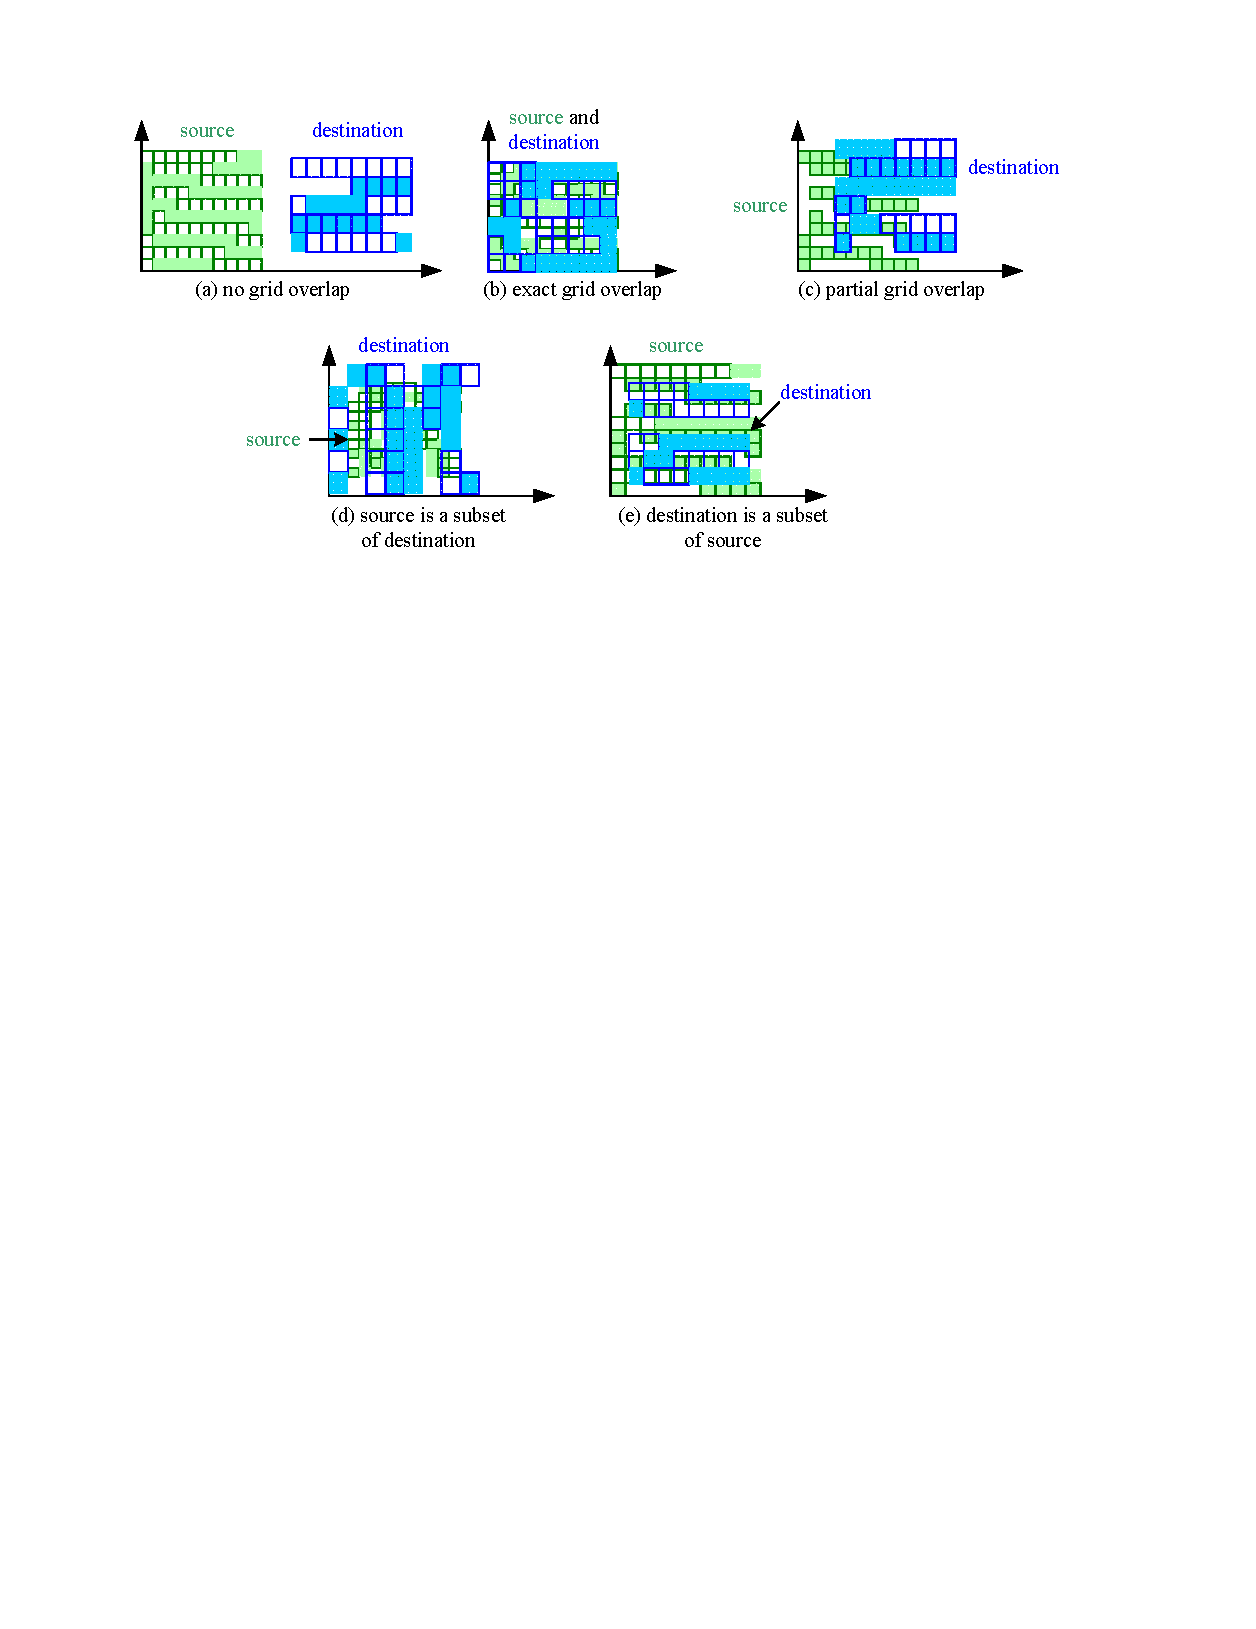
\includegraphics{RegridGridOverlap}}
\end{figure}
\end{center}

Regrid can provide complete interpolation weights for the destination Field
only for those situations where there is source data covering the entire physical
domain of the destination Grid (cases (b) and (e) above).  In all the other
cases, there are parts of the destination Grid for which there is no source. 
When source data is not available, Regrid routines will not extrapolate data
values and the destination Field may contain data points that have not been
calculated or filled.  Currently, regrid routines initialize the destination
Field to a value of zero prior to regridding, so unfilled destination data points
will have that value.  In the future, regrid routines will have an optional
argument allowing users to specify a fill value besides zero.  


\subsubsection{Regrid and Data Location}

There is no restriction in Regrid that the source and destination Fields
define their data in the same relative location (RelLoc).  However, regridding
between Fields with different RelLocs can have unintended consequences if the
related Grids cover exactly the same physical domain.  The RelLocs represent
different subGrids, which can shift the represented physical domain by plus or
minus one-half of a cell width.  This is illustrated below in Figure 
\ref{fig:RegridRelLocEffect}, which shows the physical areas described by two

\begin{center}
\begin{figure}
\caption{Illustration of Grid areas represented by differing RelLocs. }
\label{fig:RegridRelLocEffect}
\resizebox{\textwidth}{!}
  {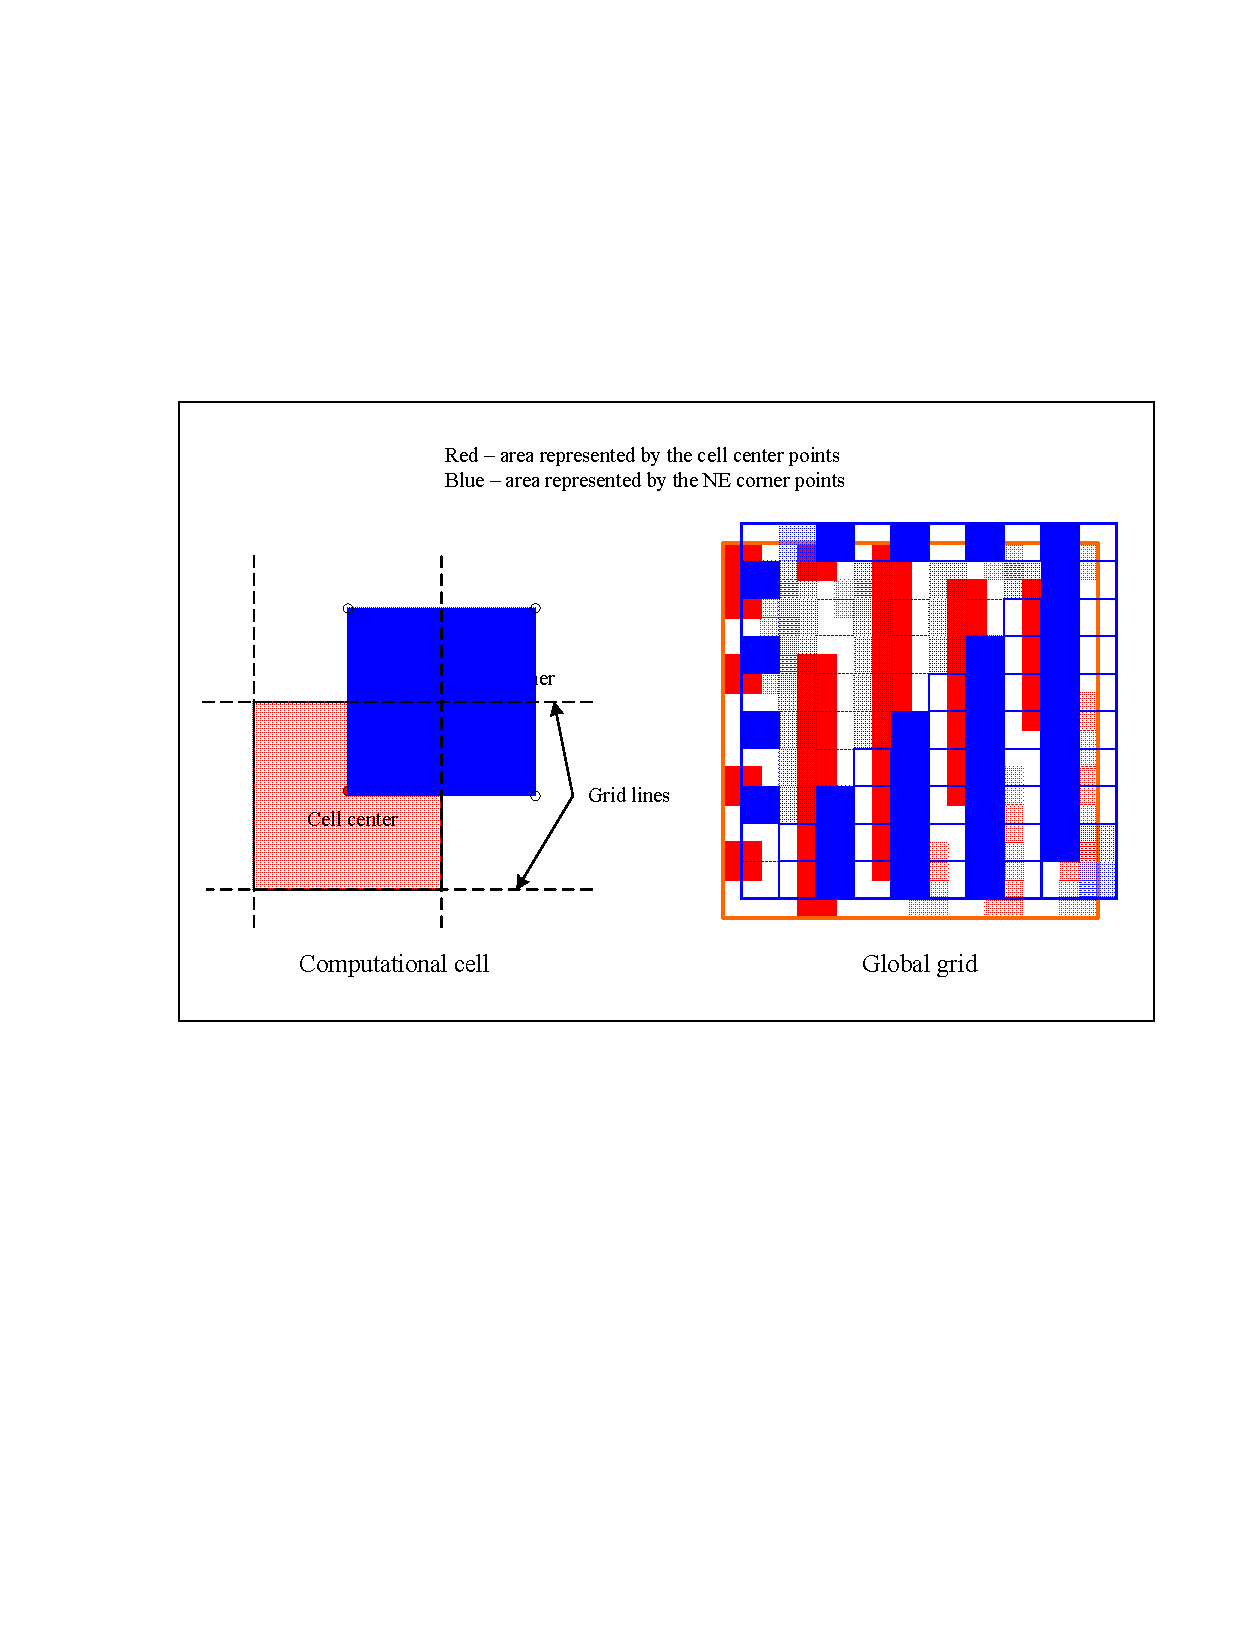
\includegraphics{RegridRelLocEffect}}
\end{figure}
\end{center}

sample RelLocs and the effect on the overlap of the global Grids.  In this
situation, there may be some unfilled or less accurate data at some of the
Grid boundaries.

Different refinement or cell sizes between the source and destination Grids
may also have a similar effect, even if their corresponding Fields have the
same RelLocs.  This is illustrated below...


\subsubsection{Regrid and Periodicity}





\subsubsection{Redist}
% $Id: ArrayRedist_desc.tex,v 1.3 2004/06/22 21:35:25 jwolfe Exp $


Redistribution operations always operate on data associated with a
single Grid, but are either decomposed across multiple processors
differently, or have different index orderings, or are decomposed
in different dimensions.  The Redistribution methods involve only
data movement; no interpolation, data binning, averaging, etc are
performed.  A typical example of Redistribution is the data transpose
associated with the translation between phycial and Fourier space.

An example of the use of ESMF Redistribution methods is presented in
the FieldRedist system test.

In the future, we plan to have specific interfaces for common uses
like the data transpose.


\subsubsection{Lower Level Functions}
The last seven correspond closely to the lower level
MPI communications primitives.  They are:
\begin{description}
\item[Gather]
Reassembling data which is decomposed over a set of DEs into a single
block of data on one DE.
\item[AllGather]
Reassembling data which is decomposed over a set of DEs into multiple
copies of a single block of data, one copy per original DE.
\item[Scatter]
Spreading an undecomposed block of data on one DE over a set of DEs,
decomposing that single block into smaller subsets of data, one
data decomposition per DE.
\item[AlltoAll]
Spreading an undecomposed block of data from multiple DEs onto
each of the other DEs in the set, resulting in a set of multiple decomposed 
data blocks per DE, one from each of the original source DEs.
\item[Broadcast]
Spreading an undecomposed block of data from one DE onto all other
DEs, where the resulting data is still undecomposed and simply
copied to all other DEs.
\item[Reduction]
Computing a single data value, e.g. the data maximum, minimum, sum, etc
from a group of decomposed data blocks across a set of DEs, where the
result is delivered to a single DE.
\item[AllReduce]
Computing a single data value, e.g. the data maximum, minimum, sum, etc
from a group of decomposed data blocks across a set of DEs, where the
result is delivered to all DEs in the set.
\end{description}

\subsection{Field and Bundle Attributes}

There are routines for setting and getting single values and lists of
int/I4, double/R8, and logical (ESMF\_Logical) types, and char */character
strings.  (Arrays of character strings are not supported.)

Attributes can be gotten by name.  The type and count can also be queried
by name and then a specific Get call can be made.  (The arguments to the
Get routines are typed and overloaded, so the type of the Attribute must
match the type of the argument receiving it.)

A count of all Attributes associated with an object can be returned, and
then Attributes can also be queried and retrieved by number, for iterating
an unknown Attribute list.

Currently Fields, Bundles, and States have Attribute support enabled.

\newpage
\subsection{Object Model}

The following is a simplified UML diagram showing the relationships among
ESMF Field, Grid and Bundle classes.  See Appendix A, {\it A Brief 
Introduction to UML},
for a translation table that lists the symbols in the diagram and their 
meaning.

\begin{center}
\includegraphics{Bundle_obj.eps}   
\end{center}









